\subsection{Emotion Recognition Chain} \label{emotion-recogniton-chain-subsec}

Die Emotion Recognition Chain (ERC) besteht aus fünf Hauptschritten: 
Datenerfassung, Vorverarbeitung, Segmentierung, Merkmalsextraktion und Klassifizierung (vgl. Abb. \ref{fig:erc}).
In den folgenden Unterkapiteln wird für jeden Schritt eine allgemeine Erklärung gegeben. \\

\todo[inline]{Artur: Need to update the erc image}

\begin{figure}[h]
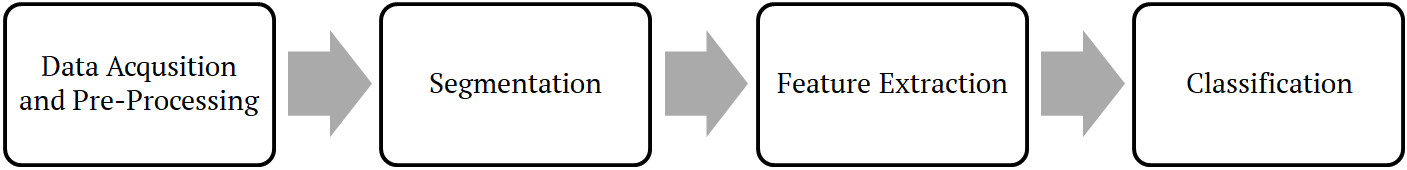
\includegraphics[width=\textwidth]{Images/erc.png} 
\vspace{-0.3cm} 
\caption{Emotion Recognition Chain: Zeitreihen-Datensätze werden von tragbaren Sensoren aufgenommen (Datenerfassung) und vorverarbeitet (Vorverarbeitung). Die Daten werden dann in Segmente unterteilt (Segmentierung), aus denen Merkmale extrahiert werden (Merkmalsextraktion). Mit den gewonnenen Merkmalen wird schließlich ein Klassifikator trainiert und anschließend dessen Ergebnisse bewertet (Klassifikation).}
\label{fig:erc} 
\end{figure} 
%\vspace{0.5cm}


% Unterkapitel 9.2.1
\subsubsection{Datenerfassung} \label{datenerfassung-subsubsec}


\todo[inline]{Artur: Später mit dem Rest der Dokumentation abstimmen.}


Dieser Schritt der ERC beinhaltet die Auswahl sowie den Aufbau der Sensoren, die Messreihendurchführung um Daten zu erhalten und Etikett-Beschriftungstechniken.
All diese Details sind wichtig für die Emotionserkennung, damit relevante und möglichst fehlerfreie Daten von Versuchspersonen für die verschiedenen emotionalen Zustände gewonnen werden können.
Dies ist besonders wichtig, da der Datenerfassungsschritt der erste in der ERC ist und die Ergebnisse aller folgenden Schritte direkt von der Qualität des Datensatzes abhängen. \\



% Vorverarbeitung, um die Daten von Rauschen zu reinigen.

% Unterkapitel 9.2.2
\subsubsection{Vorverarbeitung} \label{vorverarbeitung-subsubsec}


Normalisierungstechniken wurden auf dem gesamten Datensatz angewendet. 
Wir haben insbesondere die Standardnormalisierung verwendet, welche den Mittelwert der Daten auf Null setzt und die Einheitsvarianz ergibt \cite{grus15}. 
Die Formel für die Standardnormierung lautet:
\begin{equation} 
\Large{ {x'={\frac {x-{\overline {x}}}{\sigma }}} } 
\label{equ:norm} \end{equation} %\vspace{0.5cm}

wobei $ x $ ein Datenpunkt eines Sensorkanales, $ \overline{x} $ ist der Durchschnitt der Gesamtheit für diesen Sensorkanal und $ \sigma $ ist die entsprechende Standardabweichung.

% Unterkapitel 9.2.3
\subsubsection{Segmentation} \label{segmentation-subsubsec}


Ziel dieses Schrittes ist es, Teile von Daten zu identifizieren, welche wichtige Informationen über die zu erkennenden Emotionen enthalten. 
Dies geschieht durch Filtern der Daten und Ausschließen von Segmenten, die für das Klassifizierungsproblem nicht relevant sind.
Zusätzlich wird die zu verarbeitende Datenmenge reduziert, indem Segmente eines Zeitfensters fester Größe aus den Daten extrahiert werden.
Diese Vorgeheisweise ist heute in der Praxis besonders wichtig, da sonst hardwarebedingte Einschränkungen die zu verarbeitende Datenmenge begrenzen können. \\


In dieser Projektarbeit wurde ein Schiebefensteransatz (engl. ``sliding window approach'') verwendet. 
Ziel der Methode ist die Segmentierung der vorhandenen Daten in kleinere Einheiten, um die Merkmalsextraktion sowie die anschließende Klassifizierung zu vereinfachen oder gar erst zu ermöglichen.
Die Länge des Zeitfensters (engl. ``time window'') und des Gleitschritts (engl. ``sliding stride'') sind zu bestimmende Parameter (und werden auch als ```Hyperparameter'' bezeichnet), wobei sich das Zeitfenster auf die feste Größe pro extrahiertem Segment und der Gleitschritt auf die Lücke zwischen dem Beginn jedes Zeitfensters bezieht.
Es ist zu beachten, dass sich aufeinanderfolgende Zeitfenster überlappen können, sobald der definierte Schritt kleiner als das Zeitfenster ist. \\


Die Daten werden auf Zeitstempel-Ebene mit Etiketten beschriftet, basierend auf den von der jeweiligen Versuchsperson ausgefüllten Fragebögen. 
Jedem Zeitfenster wird ein Etikett zugeordnet, welches das dominaten (d.h. am meisten vohandene) Etikett der im Fenster enthaltenen Zeitstempel basiert. Es wird davon ausgegangen, dass jedes Zeitfenster nur von einer Emotion belegt ist. \\


\begin{figure}[h]
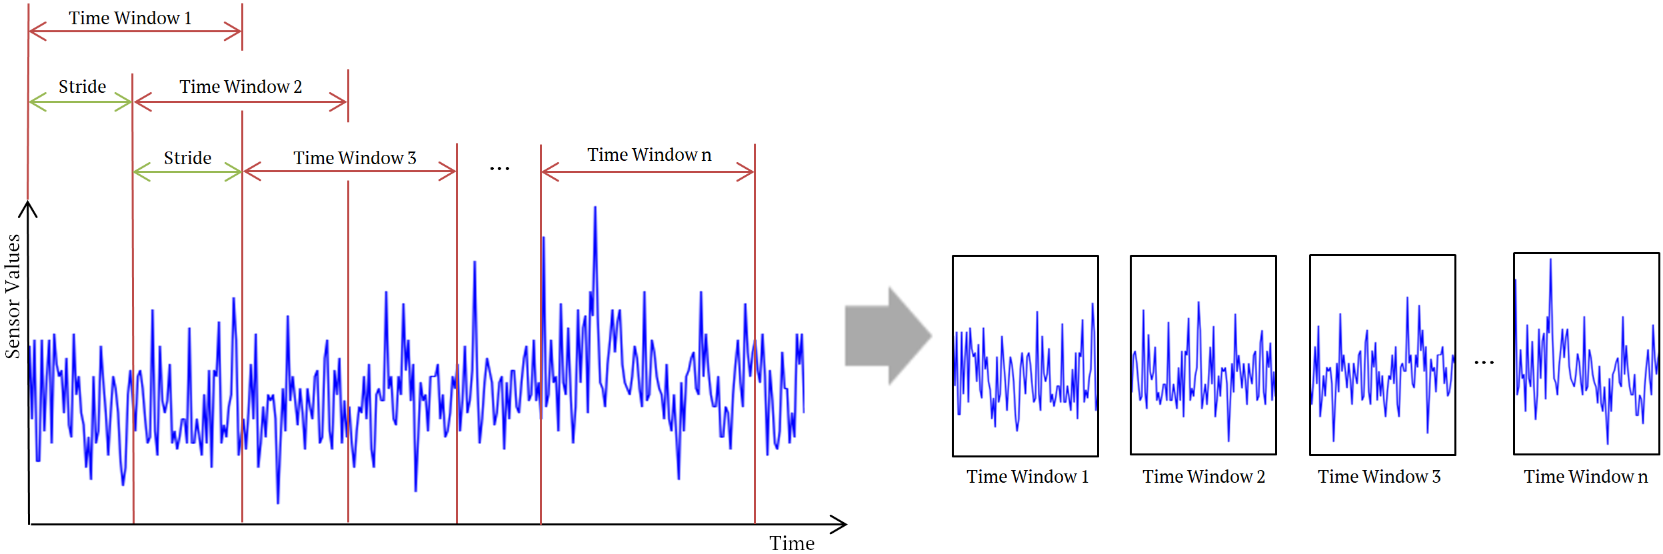
\includegraphics[width=\textwidth]{Images/segmentation.png} 
\caption{\small{Schiebefenster-Segmentierung: Die Daten werden durch ein Fenster fester Größe in kleinere Segmente aufgeteilt. Das Fenster wird mit einem festen Gleichschritt geschoben, um den aufeinanderfolgend Daten-Zeitfenster zu erhalten. }}
\end{figure} 

% Unterkapitel 9.2.4
\subsubsection{Merkmalsextraktion} \label{merkmalsextraktion-subsubsec}






% Unterkapitel 9.2.5
\subsubsection{Klassifikation} \label{klassifikation-subsubsec}





